\section{层间耦合对谱函数及能带的影响}
%\setcounter{page}{1}
%\pagestyle{plain}
 我们首先来研究2D拓扑绝缘体体态的能谱分布,在这里2D拓扑绝缘体哈密顿量是没有四重旋转对称的(也可以表示为$\mathcal{C}_4$对称)和反演对称,即
\begin{equation}
\begin{aligned}
&H_{\mathrm{TI}}(k_x,k_y)\neq H_\mathrm{TI}(-k_y,k_x)\qquad \textrm{$\mathcal{C}_4$对称破坏}\\
&H_{\mathrm{TI}}(k_x,k_y)\neq H_\mathrm{TI}(-k_x,-k_x)\qquad\textrm{反演对称破坏}\\
\end{aligned}
\end{equation}
因此,当2D拓扑绝缘体和$d$-波超导体形成异质结后,在拓扑绝缘体层通过近邻效应诱导出的电子配对也一定会破坏这两种对称性。也就是说在拓扑绝缘体中并不仅仅存在纯的$d$-波配对形式,还会存在其它对称形式的配对,这将会导致准粒子谱是不对称的。
\subsection{谱函数计算结果及分析}
 对第二章给出的模型(\ref{ham}),首先来计算不同能量下体系的谱函数。根据谱函数计算公式
\begin{equation}
A({\bf k},E)=-\frac{1}{\pi}\sum^4_{p=1}\mathrm{Im} G_{pp}({\bf k},E).
\end{equation}
这里$\mathbf{k}=(k_x,k_y)$,我们通过对能量$E$取不同的值,绘制BZ中的谱函数分布图,从结果中可以清晰的看到,当能量取不同值的时候,谱函数权重较大的位置发生了明显的变化,如图\ref{fig16}。
\begin{figure}[h]
\centering
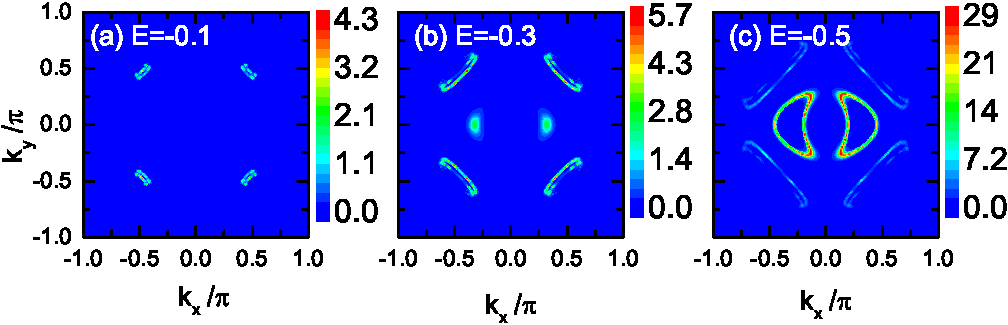
\includegraphics[scale=0.9]{pic/fig17.pdf}
\caption{2D拓扑绝缘体层谱函数强度分布。(a)$E=-0.1$,(b)$E=-0.3$,(c)$E=-0.5$}\label{fig16}
\end{figure}
计算结果显示,在低能$E=-0.1$的时候图\ref{fig16}(a),准粒子谱中在$d$-波配对的节点位置($\Delta(\mathbf{k})=0$与费米面的相交点)附近形成了小的口袋状环。这个低能的谱函数的贡献正是来自于$d$-波超导层的准粒子隧穿\cite{re59}。随着准粒子能量增加到0.3,如图\ref{fig16}(b),这个口袋的大小慢慢变大,同时在$k_y=0$的位置出也出现了另外一部分准粒子的贡献。这部分谱的权重随着能量能加变成了最大的,如图\ref{fig16}(c)所示。

 在图\ref{fig16}中有一个有趣的结果,我们发现$\mathcal{C}_4$对称性的确是被破坏了,$A(k_x,k_y)\neq A(-k_y,k_x)$,如图\ref{fig16}(b,c)所示。这个对称性被破坏的起源来自于异质结两层材料之间能带的混合,同时也与2D拓扑绝缘体中诱导出不对称的超导电子配对是有关系的。值得注意的是,在理论研究中,如果直接将一个$d$-波的超导电子配对加入到2D拓扑绝缘体的哈密顿量中,忽略两层之间的耦合,此时系统准粒子谱的$\mathcal{C}_4$对称性并未受到破坏。我们的计算结果表明,我们提出的微观模型的确可以定性的描述异质结结构的混合系统。
%==============$$==============================
\subsection{边界态计算结果及分析}
 接下来我们通过考虑一个圆柱形结构,即对于2D系统而言,一个方向是开边界的,另外一个方向是周期性边界。首先我们考虑沿$x$方向取开边界条件,沿$y$方向取周期边界条件,此时$k_y$是个好量子数,在$k_y\in\left[-\pi,\pi\right]$的区间内计算哈密顿量的本征值并得到能带图,结果如图\ref{fig17}(a)所示。这里同时包括了体态与边界态的能带,在系统的两个开放边界数,能带是有能隙的。
\begin{figure}[h]
	\centering
	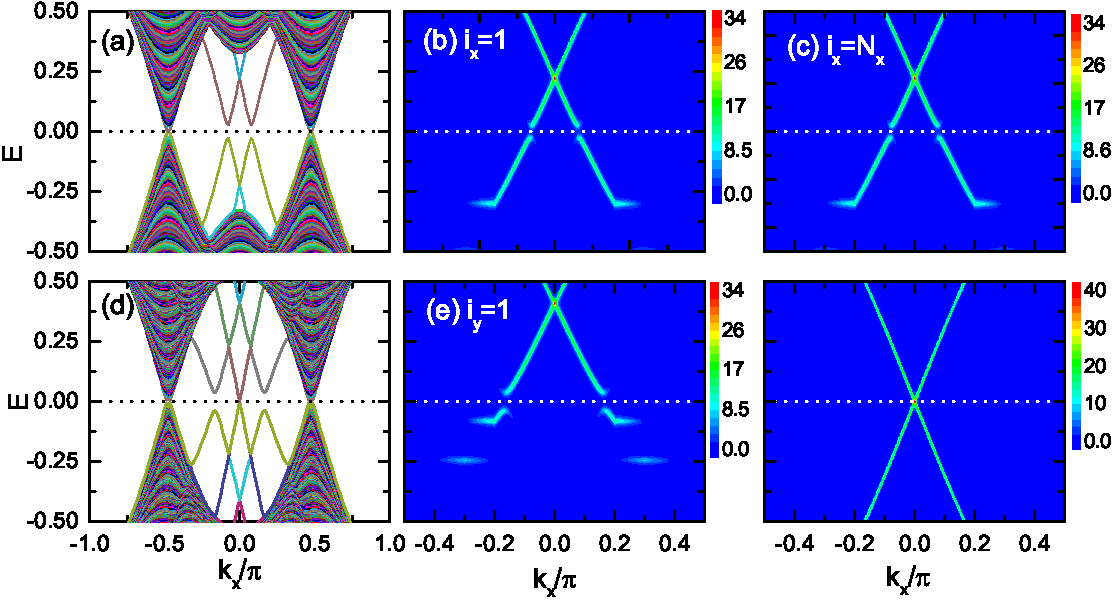
\includegraphics[scale=0.7]{pic/fig18.pdf}
	\caption{考虑圆柱形结构的数值计算结果。(a)沿$x$方向开边界时哈密顿量本征值,(b)$i_x=1$边界处的谱函数,(c)$i_x=N_x$边界处的谱函数,(d)沿$y$方向开边界时哈密顿量本征值,(b)$i_y=1$边界处的谱函数,(c)$i_y=N_y$边界处的谱函数}\label{fig17}
\end{figure}
我们同时计算了边界位置处$(i_x=1,i_x=N_x)$的谱函数,如图\ref{fig17}(b-c),从这里可以更加清晰的看到有能隙的边界态,这与能带计算得到的结论是完全相同的。从谱函数的结果中还可以看到,能隙的大小大约为0.05,这个被打开的能隙正是来源于近邻效应诱导的$d$-波配对项\cite{re27,re28}。

 我们接下讨论沿$y$方向取开边界条件的边界态。此时能带图以及格点两端($i_y=1,i_y=N_y$)的的谱函数计算结果如图\ref{fig18}(d-f)所示。此时的结果与$x$方向\ref{fig17}(a-c)中的结果是不同的,这表明体系的$\mathcal{C}_4$对称性是受到破坏的。值得注意的是此时的边界态是没有能隙的,这与之前唯象的理论模型研究的结果是不同的\cite{re27,re28}。在谱函数的计算中,两个边界处的结果也是不同的。在$i_y=1$的边界上,边界态是有能隙的,能隙大小约为0.08,这个值甚至比$i_x=1$与$i_x=N_x$边界上边界态的能隙还要大。但是在$i_y=N_y$这个边界上,边界态是没有能隙的,因此对于圆柱体结构的系统,体系的非对称性是显而易见的。此时在$i_y=N_y$这个边界上存在局域的零能边界态,这个结果可以通过实验手段进行探测。
%============================================
\subsection{局域电子态密度结果及分析}
 现在我们通过数值的方法来研究马约拉纳拐角态。我们考虑了2D拓扑绝缘体(40$\times$40的有限大小)生长在一块更大的高温超导体上,如图\ref{fig18}(a)所示。
\begin{figure}[h]
\centering
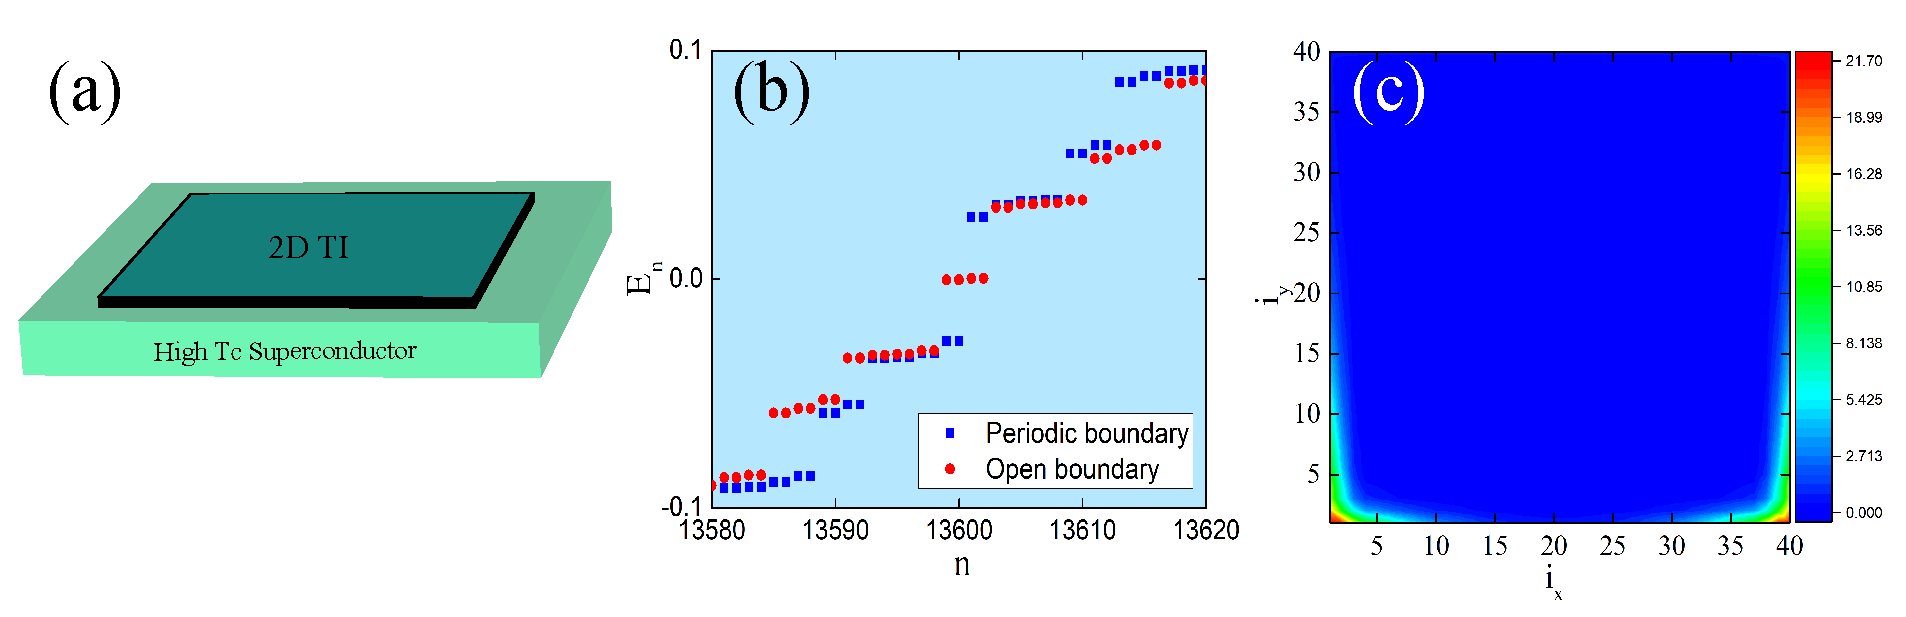
\includegraphics[scale=0.45]{pic/fig19}
\caption{(a)2D拓扑绝缘体生长在$d$-波高温超导体上,(b)实空间哈密顿量本征值(c)2D拓扑绝缘体实空间中零能态电子局域态密度}\label{fig18}
\end{figure}
首先来考虑沿$x$和$y$都取开边界条件,然后将实空间的哈密顿量矩阵对角化,得到的本征值如图\ref{fig18}(b)所示,可以看到存在四个零能本征值。当在实空间中$x$与$y$方向都取周期边界,则没有零能本征值出现。因此,这四个零能本征值是局域在边界上的,代表的是马约拉纳零能模。对于超导系统,四个零能本征值应该来源于两个零能物理的准粒子,对应着系统边界上的两对马约拉纳零能模。这两对马约拉纳零能模的空间分布可以通过计算零能本征值对应的局域电子态密度(LDOS)观测,如图\ref{fig18}(c)所示,存在两对局域在体系下边界的两个拐角处(每个拐角处存在一对)。然而在体系上边界的两个拐角处则没有零能态的存在。局域电子态密度的结果同样表明此时系统不在具有$\mathcal{C}_4$旋转对称性,而且这个对称性破坏的直接结果就是并不是每个角落里都会存在束缚态,只有在打开能隙的边界上,相邻边界之间形成质量畴壁,才可以有束缚态的存在。
%============================================
\subsection{本章总结}
 通过数值对角化矩阵的方法,我们发现了异质结耦合系统中,2D拓扑绝缘体与超导体之间耦合是比较重要的,当考虑了层间耦合时,2D拓扑绝缘体能谱的对称性会受到邻近超导层的影响,相对于唯象的将超导配对直接加入到2D拓扑绝缘体的哈密顿量中,这个微观模型可以更加正确的描述异质结系统的性质。我们同时发现不同方向上的边界态受到超导配对的影响也是不同的,这一结论从开边界时候的能带图以及边界态的谱函数计算都可以确认这一点。而从实空间LDOS的计算及第一章有效边界理论可知,此时通过近邻效应在2D拓扑绝缘体中诱导处的电子配对对称性也不再是纯$d$-波,并不是每一个边界上的边界态都会被超导诱导的电子配对打开能隙,所以在实空间中并不是每个拐角处都会出现马约拉纳束缚态,接下来我们将从动量空间以及实空间两个角度来分析这时电子配对对称性的情况。








